\documentclass{standalone}
\usepackage{pgfplots}
\pgfplotsset{soldot/.style={color=black,only marks,mark=*},
             holdot/.style={color=black,fill=white,only marks,mark=*},
             compat=1.12}
\begin{document}
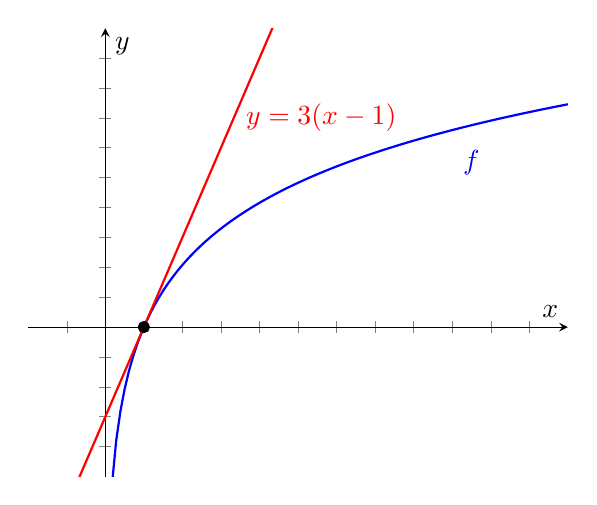
\begin{tikzpicture}
\begin{axis}[
 axis lines=middle,
 %ticklabel style={fill=blue!5!white},
 xmin=-2,xmax=12,
 ymin=-5,ymax=10,
 xtick={-1,...,1,2,3,4,...,11},xticklabels={},
 ytick={-4,...,1,2,3,4,...,9},yticklabels={},        %<--
% minor tick = {-5,-3,...,5}, %<--
 xlabel=\(x\),ylabel=\(y\),
 samples=200]

\addplot[domain=-10:12,thick,blue] {3*ln(x)};

\addplot[domain=-10:12,thick,red] {3*(x-1)};

\draw [blue] (axis cs:9.5,5.5)  node [] {$f$};
\draw [red] (axis cs:5.6,7)  node [] {$y=3(x-1)$};
\addplot[soldot] coordinates{(1,0)};

\end{axis}
\end{tikzpicture}
\end{document}